\section{Dataset}
\label{sec:dataset}

\begin{frame}
    \frametitle{FLAME Dataset Overview}

    \begin{minipage}{0.58\textwidth}
        \begin{itemize}
            \item The dataset contains \textbf{drone-captured} images of wildfires.
            \item Designed specifically for \textbf{binary wildfire classification} (\textit{Fire} vs \textit{No Fire}).
            \item \textbf{Training Set:} 39,375 images
            \item \textbf{Test Set:} 8,617 images.
            \item \textbf{Validation Split:} 10\% of training set.
            \item \textbf{Class Distribution:}
                \begin{itemize}
                    \item Fire: \textbf{25,027 images (63.55\%)}.
                    \item No-Fire: \textbf{14,357 images (36.45\%)}.
                \end{itemize}
        \end{itemize}
    \end{minipage}
    \hfill
    \begin{minipage}{0.38\textwidth}
        \begin{figure}
            \centering
            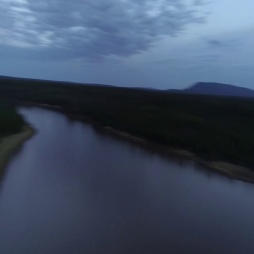
\includegraphics[width=\textwidth]{images/sample}
            \caption{Sample FLAME dataset image.}
            \label{fig:sample}
        \end{figure}
    \end{minipage}
\end{frame}